\documentclass[helvetica,narrow,openbib]{europecv}
\usepackage[T1]{fontenc}
\usepackage[a4paper,top=2cm,left=1cm,right=1cm,bottom=2cm]{geometry}
\usepackage{ifpdf}
\usepackage{bibentry}
\usepackage[italian]{babel}
\usepackage{url}
\ifpdf
    \usepackage[pdftex]{graphicx}
\else
    \usepackage{graphicx}
\fi
\usepackage{xcolor}

\renewcommand{\ttdefault}{phv} % Uses Helvetica instead of fixed width font
\renewcommand{\emph}[1]{\textbf{#1}}
\ecvlastname{Ziosi}
\ecvfirstname{Brunetto Marco}
\ecvaddress{via Ivancich n.17, 30174, Chirignago (VE)}
\ecvtelephone{(+39) 3474958152}
\ecvemail{brunetto.ziosi@gmail.com}

\ecvnationality{Italian}
\ecvdateofbirth{03/05/1985} % FIXME Solo per application in Europa

\begin{document}
\selectlanguage{italian}
\ecvfootnote{Curriculum Vitae of Brunetto Marco Ziosi}

\begin{europecv}
\ecvpersonalinfo[20pt]
\ecvitem{Website}{\texttt{brunettoziosi.eu}}
\ecvitem{LinkedIn}{\texttt{https://www.linkedin.com/in/brunettoziosi}}
\ecvitem{Public repository}{\texttt{github.com/brunetto}, \texttt{gitlab.com/brunetto}}

\ecvitem{Current Position}{\textbf{Full stack developer at Pixartprinting - a Cimpress company}}
 
\ecvsection{Education \& Employment}

\ecvitem{2015}{\emph{INAF-OAPd fellowship}: ``Study of gravitational 
waves sources in young star clusters by means of direct N-body simulations.''}

\ecvitem{}{\emph{PhD in Astrophysics}: ``The impact of stellar evolution and dynamics on the formation of compact-object binaries'' (University of Padova, funded by AACSE)}
  
\ecvitem{2011}{Master Degree Thesis in Astronomy (University of Padova)
}

\ecvitem{2007}{Bachelor Degree Thesis in Astronomy (University of Padova)}

\ecvsection{Teaching experience}
\ecvitem{2012-2013}{
\begin{itemize}\itemsep-0.1em 
\item Teaching assistant, University of Padova, Mathematical Analysys
\item Teaching assistant, University of Padova, Python course
\end{itemize}}

\ecvsection{Courses and Workshops}

\ecvitem{2016}{
\begin{itemize}\itemsep-0.1em 
\item Microservices with Docker and AWS
\item Continuous integration, Jenkins
\item Test Driven Development
\end{itemize}
}

\ecvitem{2014}{
\begin{itemize}\itemsep-0.1em 
\item Amazon Web Services Cloud School
\item Tools and Techniques for massive data analysis
\item Perspectives of GPU computing in Physics and Astrophysics
\end{itemize}
}

\ecvitem{2013}{
\begin{itemize}\itemsep-0.1em 
 \item  Workshop on High Performance Scientific Computing
 \item PhD Summer School on High Performance Scientific Computing
\end{itemize}
}
\ecvitem{2012}{
\begin{itemize}\itemsep-0.1em 
 \item Summer School of Parallel Computing
\end{itemize}
 }
 \ecvitem{2011}{
 \begin{itemize}\itemsep-0.1em 
 \item PhD Summer School on Algorithms and Architectures for Computational Science and
Engineering
 \item Workshop on Visualization of Large scientific Data
 \item Python for computational science
\item Introduction to GPGPU and CUDA
programming
\end{itemize}
}

\ecvsection{Language skills}

\ecvitem{}{Italian (Mother tongue), English (fluent)}

\ecvsection{Computer skills}
\ecvitem{OSs}{Linux, MacOS, Windows}
\ecvitem{Scripting/Programming Languages}{Go, Python, PHP, Bash, 
C/C++, Matlab/Octave, Fortran}
\ecvitem{Web}{PHP, JS, HTML5, CSS, Hugo, Nikola, Pelican, Wordpress, Blogger}
\ecvitem{Data Analysis/Plotting tools}{Veusz, Matplotlib/Pylab} 
\ecvitem{Versioning}{Git, SVN, Bazaar}
\ecvitem{Databases}{MySQL, MongoDB}
\ecvitem{Markup Languages}{LaTeX, Markdown}
\ecvitem{Graphics}{Inkscape, Gimp, ImageMagick, Blender}
\ecvitem{Presentation}{Beamer, Sozi/Inkscape, Prezi, PowerPoint, Javascript based (Remark)}
\ecvitem{Office/Internet}{MSOffice, LibreOffice/OpenOffice, Chrome, Internet Explorer, Firefox, Opera, Outlook, Thuderbird}

\ecvsection{Other interests}
\ecvitem{}{

Volunteering with A.G.E.S.C.I. (Wood Badge 17/03/2012-356) and Protezione Civile (Civil Defense)

Digital Photograpy

Piano and guitar

Travelling

Mapping and geo-data manipulation (OpenStreetMap project)
}

\ecvsection{Signature}
\ecvitem{}{
\begin{flushright}
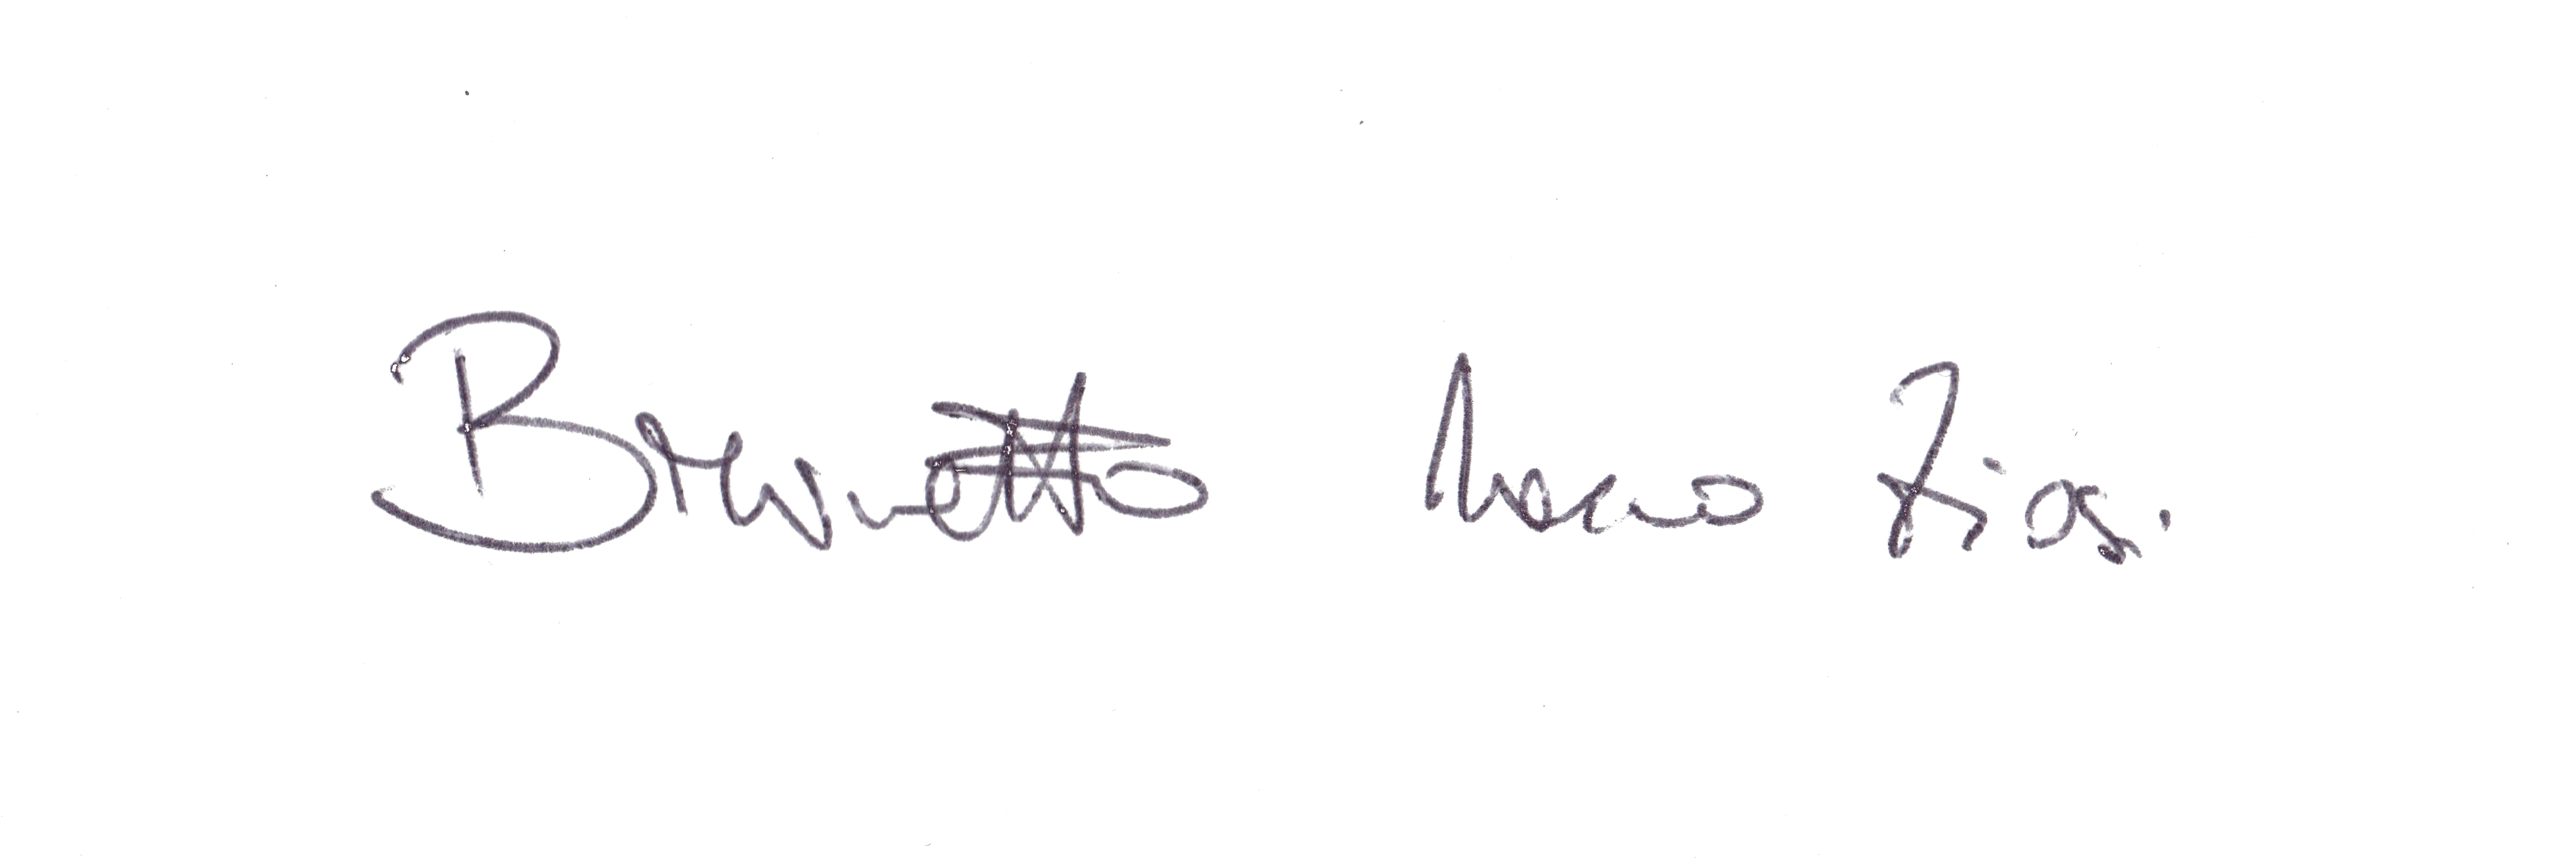
\includegraphics[width=9cm]{firma}
\end{flushright}
}

\end{europecv}
\end{document} 
